\documentclass[a4paper, 11pt, twocolumn]{article}

\usepackage[a4paper, total={6.24in, 8.5in}]{geometry}
\usepackage[utf8]{inputenc}
\usepackage{graphicx}
\usepackage{verbatim}
\usepackage{float}
\usepackage{array}
\usepackage{xfrac}
\usepackage{mathpazo}
\usepackage{amsmath}
\usepackage{bm}
\usepackage{multirow}
\usepackage{makecell}
\usepackage{multicol}
\usepackage{sectsty,textcase}
\usepackage{wrapfig,lipsum,booktabs}
\usepackage{enumitem}
\usepackage{hyperref}
\usepackage{makecell}
\usepackage{array}
\usepackage{layouts}

\bibliographystyle{plain}
\renewcommand{\thesection}{\arabic{section}}
\setlength{\columnsep}{15pt}
\newcommand{\myparagraph}[1]{\paragraph{#1}\mbox{}\\}

\title{FYS-STK3155/4155 Applied Data Analysis and Machine Learning - Project 3 }

\author{Lotsberg, Bernhard Nornes \\ Nguyen, Anh-Nguyet Lise \and
\url{https://github.com/liseanh/FYS-STK4155-project3}}
\date{November - December 2019}
\begin{document}
\twocolumn[
  \begin{@twocolumnfalse}
    \maketitle
    \begin{abstract}
		Whole page: \printinunitsof{in}\prntlen{\textwidth}
		Column: \printinunitsof{in}\prntlen{\columnwidth}
	\end{abstract}
  \end{@twocolumnfalse}
]


\section{Introduction}
In popular culture the neural network is probably the most well known form of machine learning.
 In recent years many other statistical learning methods have proven themselves
 as well however.
 In this project we compare the performance of neural networks and gradient boosting in the case of binary classification.
 In addition to these, we also use the much simpler k-nearest neighbours method as a baseline for classification performance.



\section{Data}

The data set we will analyse in this project is the MAGIC Gamma Telescope data
set retrieved from the \href{https://archive.ics.uci.edu/ml/datasets/MAGIC+Gamma
+Telescope}{UCI Machine Learning Repository}, which was generated by a Monte
Carlo (MC) program described by D. Heck et. al. \cite{heck1998corsika} to
simulate high energy gamma particle registration in a Cherenkov gamma telescope.
The set consists of ten explanatory variables and a binary response variable
\texttt{class} which specifies whether the measured photons resulted from a gamma
particle (\texttt{class} = g) or a hadron (\texttt{class} = h). The entire data
set consists of 19020 instances with no missing values, with outcome distribution
as shown in Figure \ref{fig:Histogram}. The explanatory and response variables
are defined as the following by the UCI Machine Learning Repository
\cite{Dua:2019}:
\begin{enumerate}[leftmargin=5mm, itemsep=0pt,  parsep=1pt]
  \item \texttt{fLength}: continuous \# major axis of ellipse [mm]
  \item \texttt{fWidth}: continuous \# minor axis of ellipse [mm]
  \item \texttt{fSize}: continuous \# 10-log of sum of content of all pixels
        [in \#phot]
  \item \texttt{fConc}: continuous \# ratio of sum of two highest pixels over
        fSize [ratio]
  \item \texttt{fConc1}: continuous \# ratio of highest pixel over fSize [ratio]
  \item \texttt{fAsym}: continuous \# distance from highest pixel to center,
        projected onto major axis [mm]
  \item \texttt{fM3Long}: continuous \# 3rd root of third moment along major
        axis [mm]
  \item \texttt{fM3Trans}: continuous \# 3rd root of third moment along minor
        axis [mm]
  \item \texttt{fAlpha}: continuous \# angle of major axis with vector to origin
        [deg]
  \item \texttt{fDist}: continuous \# distance from origin to center of ellipse
  [mm]
  \item \texttt{class}: g, h \# gamma (signal), hadron (background)
\end{enumerate}


\begin{figure}
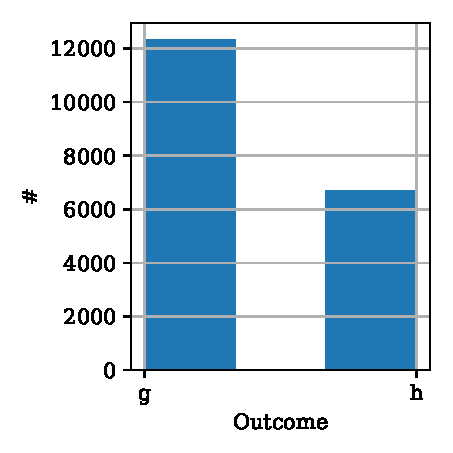
\includegraphics[scale=1]{{figures/histogram}.pdf}
\caption{Frequencies of the outcomes g and h in the data set. The numbers of
instances for the categories were 12332 and 6688 for g and h respectively.}
\label{fig:Histogram}
\end{figure}

\begin{figure*}
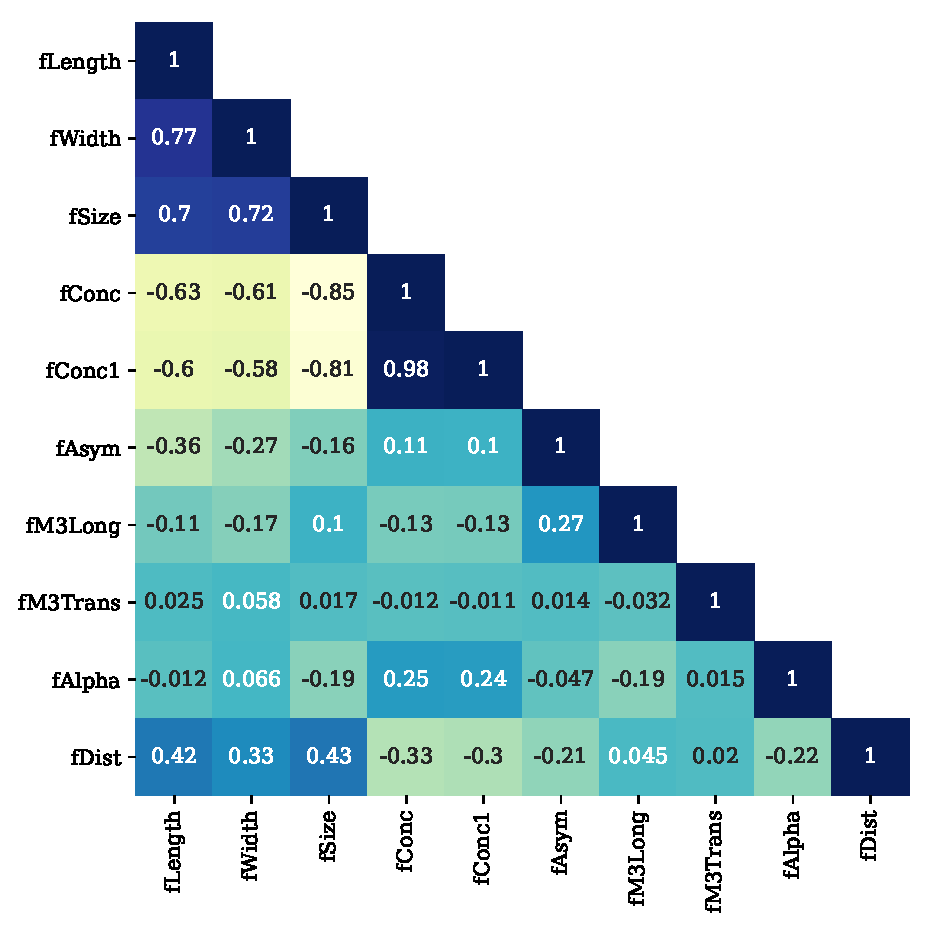
\includegraphics[scale=1]{{figures/correlation_matrix_train}.pdf}
\caption{Correlation matrix of the features in the train set. Upper triangle
excluded for readability.}
\label{fig:Correlation}
\end{figure*}
\section{Method}

\section{Results}

\begin{figure*}
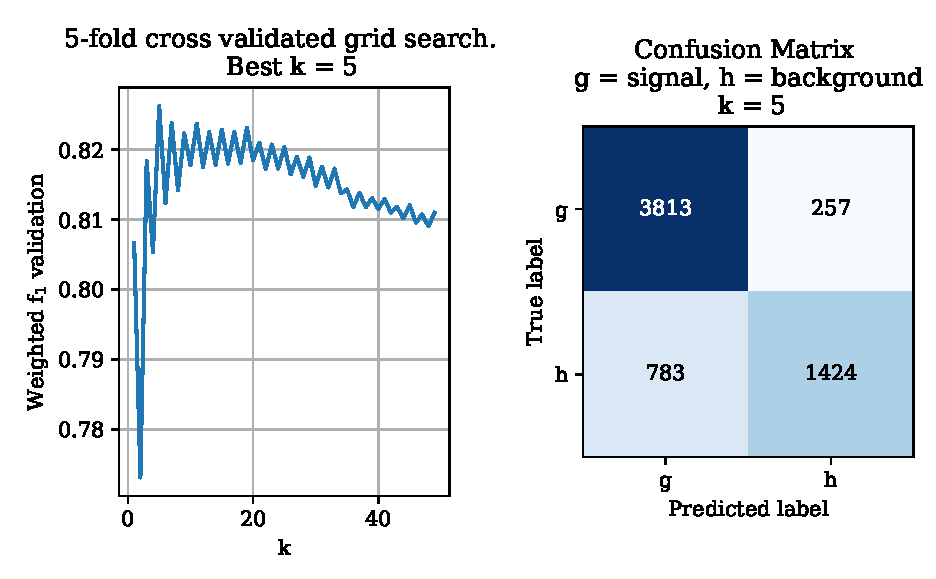
\includegraphics[scale=1]{{figures/kNN_cv_results}.pdf}
\caption{Results from tuned kNN using cross validation. The confusion matrix was
found using the test set.}
\label{fig:kNN}
\end{figure*}

\begin{figure}
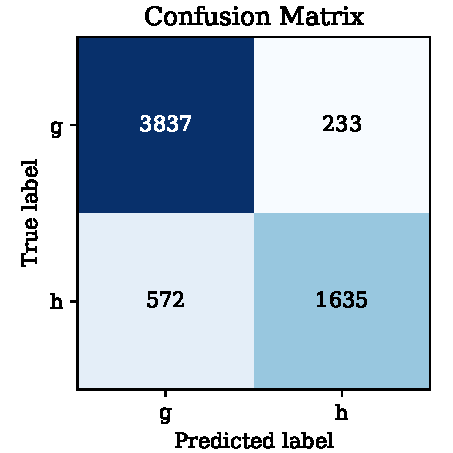
\includegraphics[scale=1]{{figures/nn_confusion_matrix}.pdf}
\caption{Confusion matrix of the neural network model applied to the test set.}
\label{fig:NN_confusion}
\end{figure}

\begin{figure}
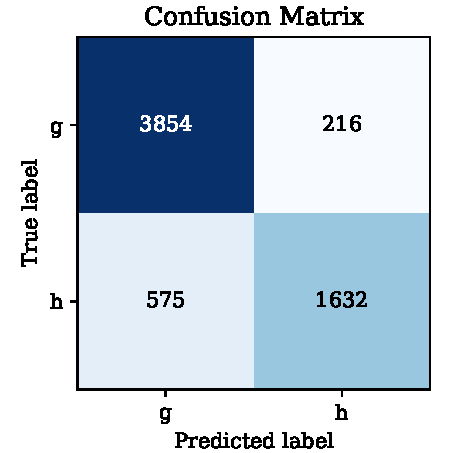
\includegraphics[scale=1]{{figures/xgboost_confusion_matrix}.pdf}
\caption{Confusion matrix of the gradient boosted model applied to the test set.}
\label{fig:XGB_confusion}
\end{figure}

\section{Discussion}

\section{Conclusion}

%\bibliographystyle{iEEEtran}
\bibliography{bibliography}



\end{document}
